\chapter{Project Management Documents}
\settocdepth{chapter}


\section{Group Contract}
\label{group_contract}

\begin{figure}[H]
\centering
    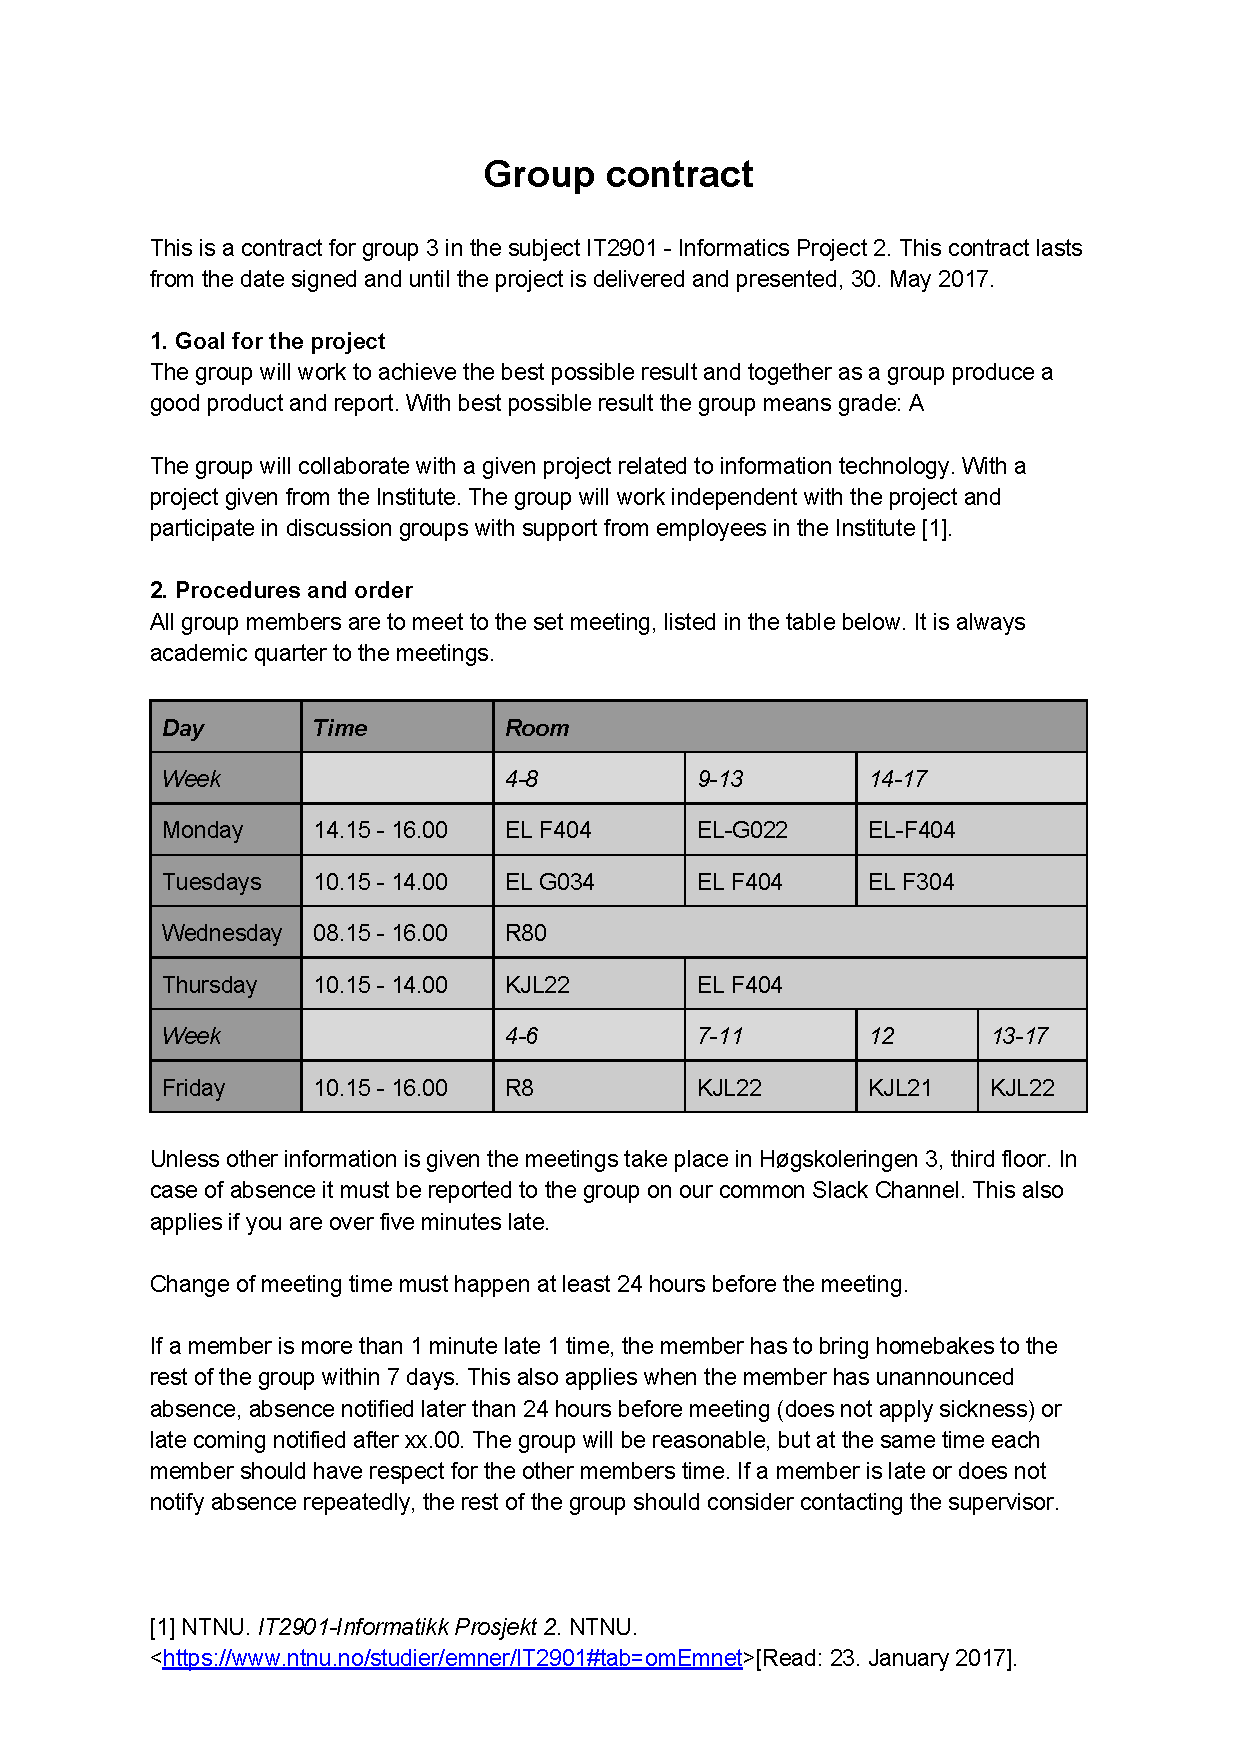
\includegraphics[width=0.85\textwidth]{fig/GroupContract1.pdf}
    \caption{Group contract page one}
    \label{Group_Contract_1}
\end{figure}

\begin{figure}[H]
\centering
    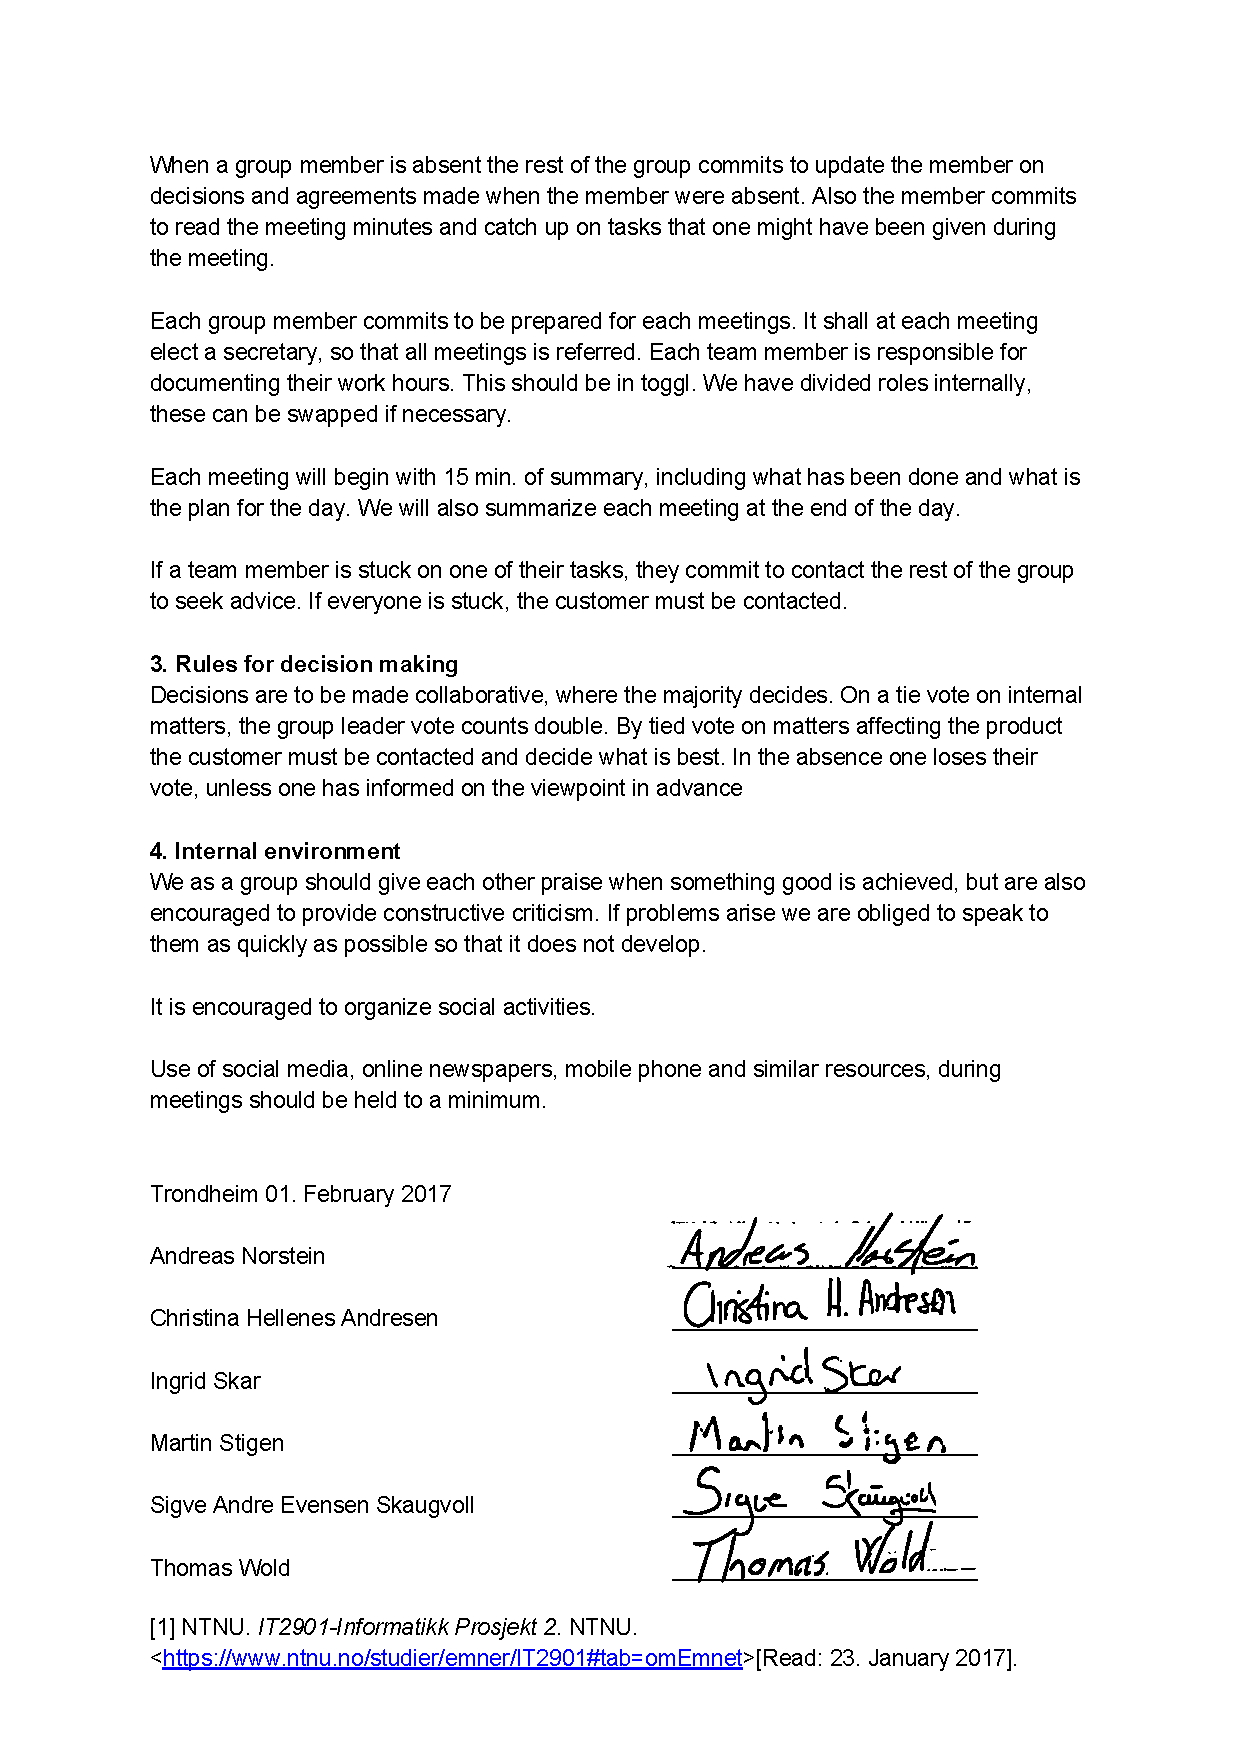
\includegraphics[width=0.85\textwidth]{fig/GroupContract2.pdf}
    \caption{Group contract page two}
    \label{Group_Contract_2}
\end{figure}

\section{Customer Contract}
\label{customer_contract}

\begin{figure}[H]
\centering
    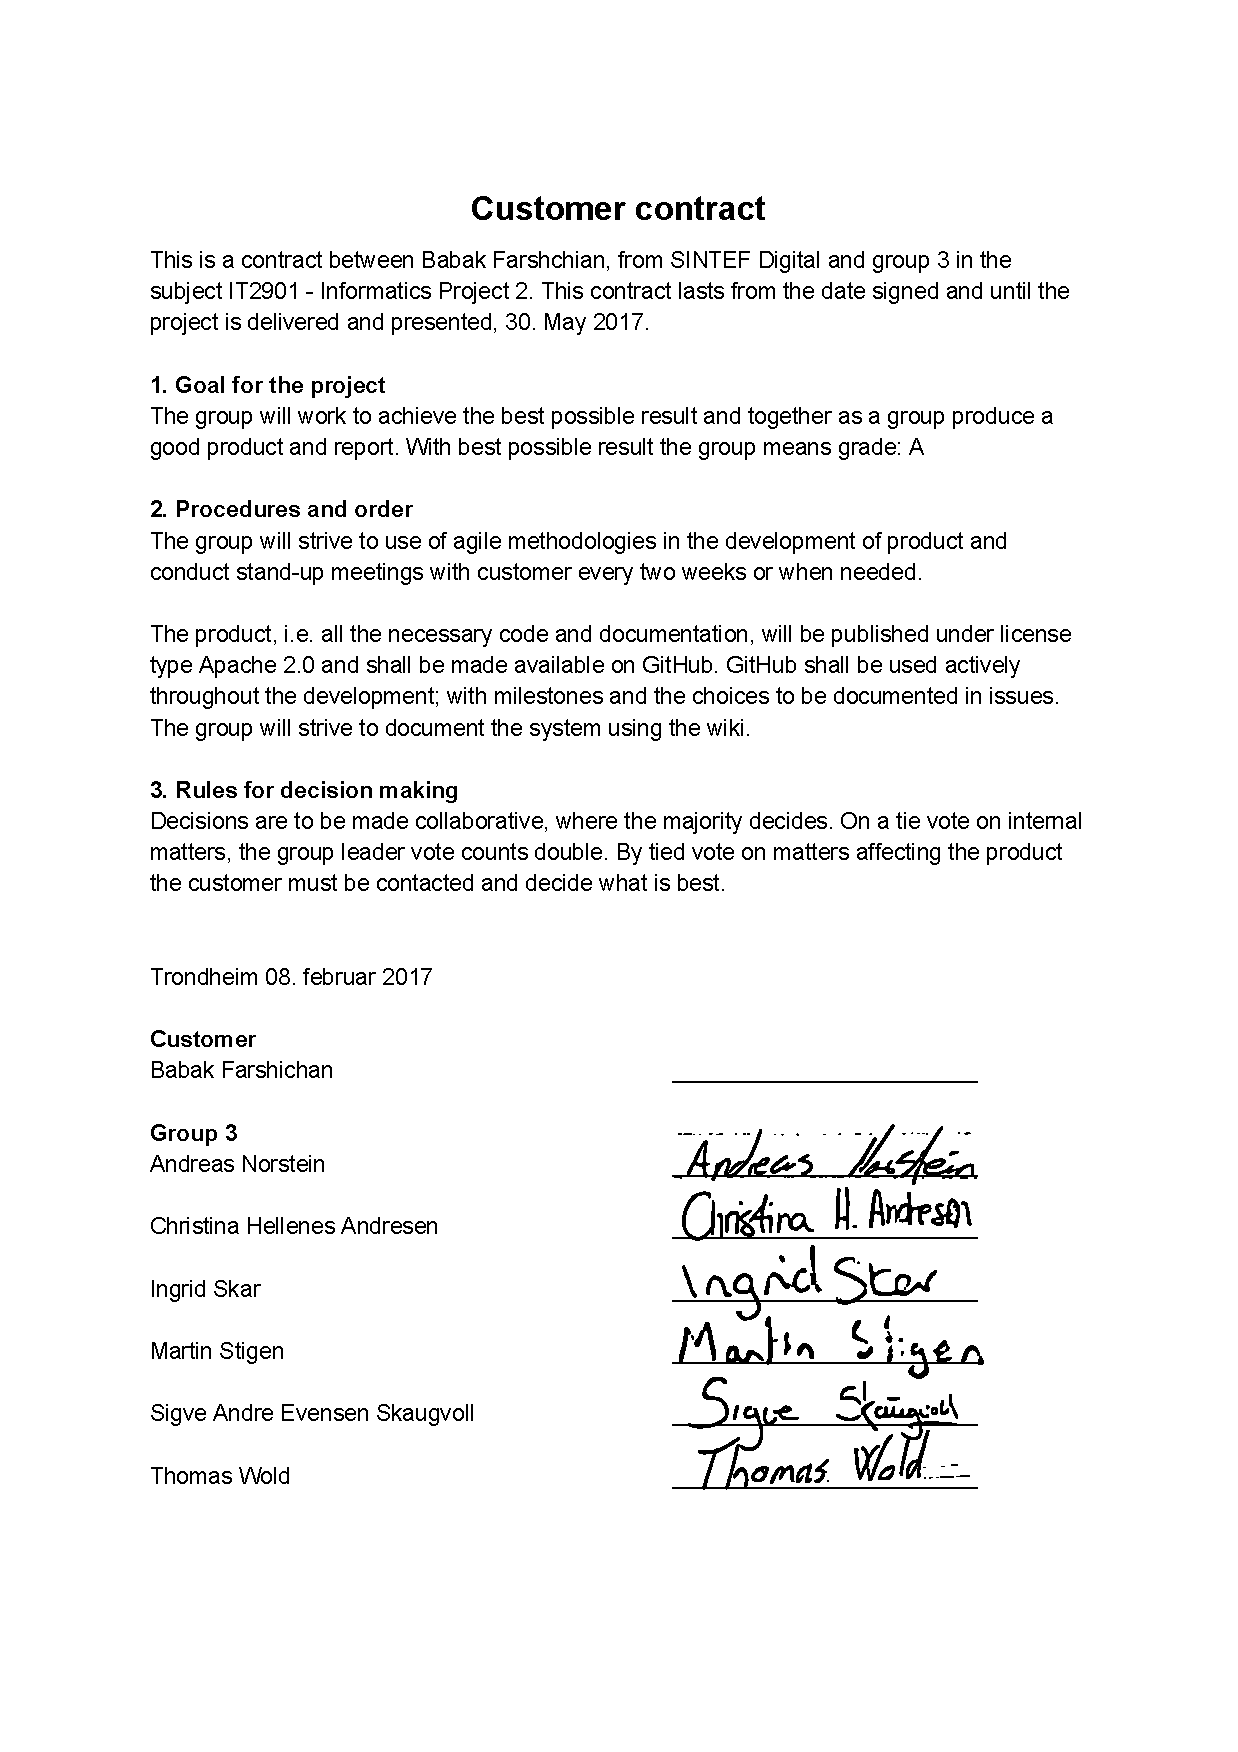
\includegraphics[width=0.85\textwidth]{fig/CustomerContract.pdf}
    \caption{Customer contract}
    \label{Customer_Contreact}
\end{figure}

\section{Meeting Minutes Daily Meetings}
\label{meeting_minutes_daily_meetings}

An example of meeting minutes from sprint 2. 

{\huge{07.03.2017}}\\
\textbf{Tilstede:} Martin, Sigve, Thomas, Ingrid, Andreas, Christina\\
\textbf{Ikke tilstede:} Ingen\\
\textbf{Arbeidstid:} 10:15 - 14:00\\
\textbf{Kakestraff:} Ingen \\

{\Large{Agenda}}
\begin{itemize} 
    \item Sende møteagenda til Babak
    \item Spørsmål om Security - Privacy
    \item Flytdiagram
    \item Domenekjøp
    \item Unit tester
\end{itemize}


{\Large{Siden sist}}
\begin{itemize}  
    \item \textbf{Thomas:} Leste over rapport i går
    \item \textbf{Ingrid:} Begynt å skrive om til Redux
    \item \textbf{Martin:} Gjøre formet for å lage aktiviteter litt bedre og se på å legge til bilde fra instagram
    \item \textbf{Andreas:} Fikse ferdig logg inn og hvor du bli redirected når du logger inn
    \item \textbf{Sigve:} Begynte å se på testing
    \item \textbf{Christina:} Jobbet med test caser og skrevet rapport.
\end{itemize}


{\Large{Dagen i dag}}\\
{\large{Sende møteagenda til Babak}}
\begin{itemize}  
    \item Vise frem prototype (siste dev.)
    \item Hvordan gikk det hos Helsedirektoratet, noen tilbakemeldinger?
    \item Har dere noe informasjon som vi kan få om hvordan utføre akseptansetest?
\end{itemize}

{\large{Spørsmål om Security - Privacy}}
\begin{itemize}  
    \item Vi venter litt med det. Er snakk om at sensitive data ikke skal deles.
\end{itemize}

{\large{Flytdiagram}}
\begin{itemize}  
    \item Endre farge på pilene, og farge på flytdiagrammet.
\end{itemize}

{\large{Domenekjøp}}
\begin{itemize}  
    \item Kanskje to linjer om det, men ikke nødvendigvis noe vi trenger.
\end{itemize}

{\large{Unit-tester}}
\begin{itemize}  
    \item Vi er litt uenige, alle tenker det er lurt.
    \item Siden kunden ikke ønsker at vi skal bruke tid på det, bestemmer vi oss for å ikke lage det.
\end{itemize}




\section{Meeting Minutes Customer Meetings}
\label{meeting_minutes_customer_meetings}

An example of meeting minutes from a meeting with customer.

{\huge{05.04.2017}}\\
\textbf{Tilstede:} Babak Farshchian, Martin, Sigve, Thomas, Ingrid, Andreas, Christina\\

{\Large{Agenda}}
\begin{itemize} 
    \item Vise frem siste prototype
    \item Fokusgruppetest
\end{itemize} 


{\large{Prototype}}
\begin{itemize}  
    \item Lage en knapp som vi viser om brukeren har registrert seg på skalvi.no eller ikke.
    \item Legge til søkefelt om å søke på tilrettelegging i aktører.
    \item Legge i backlog at man skal kunne legge til tilrettelegging når man lager en bruker
    \item Fiks tid på modalen
    \item Hvis man legger til et Facebook aktivitet som allerede ligger der burde man få en beskjed om at det ligger på siden vår fra før av.
\end{itemize}

{\large{Fokusgruppetest}} \\
Rolf fra KUBA, som vil legge inn arrangementer kommer og en til som jobber med aktørbasen, han vil se at det han gjør kan brukes
\begin{itemize}  
    \item 10 min intro
    \item 10 min på demo
    \item 40 min diskusjon
    \item Ligner på fritiden min, men den er forskjellig fordi vi har… : bygd på aktør database dataene, kan hente informasjon fra Facebook og instagram. Vi har løst problemet og det er kjempeenkelt.
    \item Aktørene må ikke komme inn legge til aktiviteter, foreldre kan også legge til aktiviteter 
    \item Ha spørsmålene vår til dem klare
    \item Hvor lett syns Rolf det er å legge til aktiviteter her, kontra det han har i dag. Tror du at andre som skal bruke dette vil være nyttig.
    \item Registrere en aktør og en bruker hos oss.
    \item Hva syns det om arrangør begrepet? Forklar hva vi mener, at alle kan foreslå arrangører. Vi må ha et eksempel: lag et case som vi bruker som senario og gi dem muligheten til å tenke rundt det.
    \item Styrken er at det er fleksibelt, alle kan foreslå arrangører.
    \item Et scenario med å lage Facebook aktivitet.
    \item Vi kan lage en liste med ting vi kunne ønsket oss i aktørbasen
    \item At aktørbasen inneholder informasjon om aktiviteter de tilbyr, flere felt burde bli fylt ut, ikke bare at navn blir registrer, det ligger noe informasjon om tilrettelegging de tilbyr.
    \item Lag en begreps slide, som definerer alle begrepene vi bruker
    \item Hva tenker dere om hvem som skal jobbe videre med prosjektet, hvordan “tjene” penger på dette.
\end{itemize}


\section{Meeting Minutes Supervisor Meetings}
\label{meeting_minutes_supervisor_meetings}

An example of meeting minutes from with supervisor.

{\huge{04.04.2017}}\\
\textbf{Tilstede:} Sofia Papavlasopoulou, Martin, Sigve, Thomas, Ingrid, Andreas, Christina\\


{\Large{Agenda}}
\begin{itemize} 
    \item Stand up
    \item Answer to our questions
\end{itemize} 

{\large{Prototype}}
\begin{itemize}  
    \item All are going well and we are soon to be finished with the product. om å søke på tilrettelegging i aktører.
\end{itemize}

{\large{Answer to our questions}}
\begin{itemize}  
    \item Activity plan: Is nice because it is a representation of how we have worked. Can use github, but we need to represent it in one way.
    \item User stories: We need functional requirements, Terje said we did not need to create use cases if we did not use them. This is okay for Sofia as well.
    \item What to call the section: May be our solution or move to pre studies
    \item Prestudy and introduction: Why we are different from other solutions can fit here, maybe. Why they should use our system, this is what we have learned from others and extract inspirations and then tell what we are different. Not very technical, more generic. Should split up prestudy to product and process
    \item Should focus on changing the things we got feedback on and then add new things and change other things.
\end{itemize}

{\large{Presenting our product}}
\begin{itemize}  
    \item Planning to have a presentation at 11th may in Drivhuset. 5 min presentation and 1 min pitch.
    \item Optionally a poster, they are only providing table and pads. Can have poster, flyers, presentations. Personal opinion to Sofia is poster, it is nice and easy to see. 
    \item We can get help if we need to print something.
    \item We can show whatever we want. 
    \item We can invite whoever we want.
    \item Presentations is part of the grade in general. Not grade the skills on presentation, not how, but what you present. Good to make an effort.
Can split up so everyone don’t need to stand on the stand the whole two hours.
\end{itemize}

{\large{Next meeting}}
\begin{itemize}  
    \item Now its easter, and Sofia is away from 24-28. April. But we can send any information we want. 
    \item We have only one final meeting, we will set the date. We do not need it, but if we want we can. 
    \item The best is to set it early and in the beginning of may, otherwise she is flexible. 
\end{itemize}


\section{Status Report}
\label{status_report}

An example of status report sent bi-weekly to supervisor.

{\Large{Week 12 and 13}}\\

{\large{1 Introduction}}\\
The past two weeks the group has only worked on the product. We have caught up on all work and are planning to have code freeze at the 7th of April.			
{\large{2 Progress summary}}\\					
We are now in the middle of sprint 4, and have only minor tasks left for the next week. We have not encountered any problems in the last two weeks and are working well as a team.  We had planned together with the customer to do user tests in the past weeks, but it has been postponed, hopefully we are able to do them next week. Therefore we might have to use some time after easter to fix things and have code review. 

We have implemented the functionality where users can give feedback on activity. The customer also wanted us to implement a page where you can get information about activity providers in Trondheim, this has also been done in the past week.

You can see the product on www.skalvi.no if you want to see how we are doing. 

The group has now displayed overall six prototype versions to the customer. 

{\large{3 Open / closed problems}}\\
At this time of the development process there are no open problems within the group or in the project.

{\large{4 Planned work for next period}}\\
For the next period we hope to finish our product, and have user testing and code review. We are also going to use time on the report, and update with the feedback we got.

{\large{5 Updated risks analysis}}\\
We have lost some resources due to sickness this week, but we do not need to update our risk analysis, since we already have thought of this problem. The rest of the group are being productive.

\section{Final Risk Analysis}
\label{final_risk_analysis}

\cleardoublepage